\documentclass[a4paper]{article}
\usepackage[parfill]{parskip}
\usepackage{fullpage}
\usepackage{enumitem}
\usepackage{hyperref}
\usepackage{blindtext}
\usepackage{multicol}
\usepackage{siunitx}
\usepackage{graphicx}
\bibliographystyle{plain}


\begin{document}

\centerline{\large NLP Assignment 2}
\vspace{0.2in}
\centerline{\Large\bf SVM-based Sentiment Detection of Reviews}
\vspace{0.1in}
\centerline{\large {Anik Roy, Christ's (ar899)}}
\vspace{0.1in}
\centerline{\large {\today}}
\vspace{0.05in}
\centerline{Word Count: 918\footnote{Using texcount}}
\vspace{0.2in}


\begin{multicols}{2}
  
\section{Introduction}

Support vector machines are an ML model which can be used to classify vectors in a vector space. This method can be applied to the task of classifying documents by representing each document as a vector. In this report, I use a neural model, doc2vec, introduced by Mikolov and Le \cite{DBLP:journals/corr/LeM14}, in order to generate feature vectors. We also qualitatively show that the vector space produced by the doc2vec model is meaningful, by examining the behaviour of document embedding generation by doc2vec.

\section{Background}

In a previous report, I used a bag of n-grams representation for documents (BOW), and used an SVM to classify these feature vectors. In BOW, each document is represented by a feature-count vector $(n_1(d), \dots ,n_m(d))$, with $n_i(d)$ being the number of occurrences of $f_i$ in $d$. I also trained on representation only using the presence of n-grams, setting $n_i(d)$ to 1 if $f_i$ appeared in $d$, and 0 otherwise.

\subsection{Support Vector Machines}

SVMs are supervised learning models which are used to classify feature vectors in an n-dimensional space. Training consists of finding a hyperplane which separates the two classes with the largest margin. Classification takes place by measuring the distance of feature vectors to the plane. 

\subsection{Doc2Vec}

Doc2Vec is an unsupervised model for learning document embeddings which can be used as feature representations. It tries to overcome two flaws in BOW - word order is not being taken into account, and semantically similar words being equidistant. Doc2Vec produces fixed-length vectors for decuments of any length. An important feature of these vectors is that they can't be directly interpreted.

Doc2Vec extends word2vec \cite{DBLP:journals/corr/MikolovSCCD13} , a method of learning word embeddings. There are two doc2vec architectures, distributed bag of words (DBOW) and distributed memory (dm).

\section{Method}

I used the doc2vec implementation found in gensim \cite{gensim} and the SVMlight \footnote{http://svmlight.joachims.org/} SVM implementation. I used the Stanford Large Movie Review Dataset \cite{maas-EtAl:2011:ACL-HLT2011} in order to train the doc2vec model. This contains 50,000 labelled (balanced) reviews and 50,000 unlabelled. I performed tokenization using the nltk package \footnote{https://www.nltk.org/api/nltk.tokenize.html} \cite{bird-loper-2004-nltk}. I also used a smaller labelled and balanced dataset of 2000 reviews, a modificaion of the reviews used by Pang et al. \cite{pang2002thumbs}, given to us in the framework of an NLP course.

I used the smaller dataset to train the SVM classifier, performing a 10-fold round-robin stratified cross-validation. 

To tune parameters for the doc2vec model, I used a 10\% validation set to evaluate different doc2vec hyperparameters. I employed a naïve search strategy, starting from the parameters used by Lau and Baldwin \cite{lau2016empirical}. After finding the hyperparameters which gave the highest accuracy on the validation set, I discarded all other models.

I compare the doc2vec based SVM model to two baseline svm models using a BOW representation.

\section{Results}

\begin{table*}
  \centering
  \begin{tabular}{llllllll}
  Method & Vector Size & Window Size & Min Count & Epochs & Hierachical Softmax &  &  \\ \cline{1-6}
  DBOW   & 120         & 7           & 15        & 5      & True                &  & 
  \end{tabular}
  \caption{Values for the optimal hyperparameters found for the doc2vec model}
  \label{tab:param-tab}
\end{table*}



\begin{table*}
    \centering
    \begin{tabular}{lllll}
    \cline{1-4}
    \multicolumn{1}{|l|}{}            & \multicolumn{1}{l|}{BOW - freq.} & \multicolumn{1}{l|}{BOW - pres.} & \multicolumn{1}{l|}{Doc2vec} &  \\ \cline{1-4}
    \multicolumn{1}{|l|}{Doc2vec}     & \multicolumn{1}{l|}{\num{1.40e-4}}       & \multicolumn{1.83e-4}{l|}{0.002}       & \multicolumn{1}{l|}{-}       &  \\ \cline{1-4}
    \multicolumn{1}{|l|}{BOW - pres.} & \multicolumn{1}{l|}{\num{1.00e-3}}       & \multicolumn{1}{l|}{-}           &                              &  \\ \cline{1-3}
    \multicolumn{1}{|l|}{BOW - freq.} & \multicolumn{1}{l|}{-}           &                                  &                              &  \\ \cline{1-2}
                                      &                                  &                                  &                              & 
    \end{tabular}
    \caption{Comparing SVM systems: p-values, using a monte-carlo permuation test with $\alpha=0.05$}
    \label{tab:pval-table}

\end{table*}

\begin{table*}
    \centering
    \begin{tabular}{|l|l|l|}
    \hline
      & Representation  & Accuracy \\ \hline
    A & BOW - frequency &  73.3    \\ \hline
    B & BOW - presence  &  86.3    \\ \hline
    C & Doc2vec         &  88.2    \\ \hline
    \end{tabular}
    \caption{Accuracies, using ten-fold cross validation over 1800 reviews}
    \label{tab:acc-table}
\end{table*}

The best parameters found for the doc2vec model are shown in \ref{tab:param-tab}, acheiving an accuracy of 86\% on the validation set. I also set the parameter dbow\_words in order to learn individual word vectors alongside document vectors. I found that the DM architecture was not as effective as the DBOW architecture.

The results of then evaluating the systems under cross-validation (not using the validation set), show that the doc2vec representation is significantly better than either of the bag of words representations when using an SVM.

\section{Analysis}

Since doc2vec vectors are not directly interpretable, we have to analyse document embeddings to attempt to see what the model is doing. 

\begin{figure*}
  \centering
  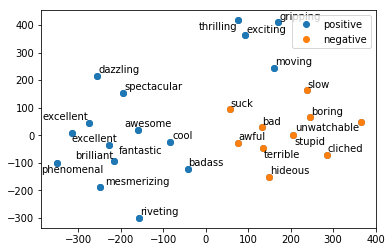
\includegraphics{figs/adjectives.png}
  \caption{Plot of deviation from the mean of word vector components}
  \label{fig:adj-fig}
\end{figure*}

Since word embeddings were also learned by the DBOW model, I look at word vectors generated for a variety of  for positive and negative adjectives. Figure \ref{fig:adj-fig} shows a t-SNE projection \cite{maaten2008visualizing} of embeddings for sentiment words suggested by Pang et al. \cite{pang2002thumbs}. The negative words are grouped, suggesting that the model learns the sentiment of individual words.

\begin{figure*}
  \centering
  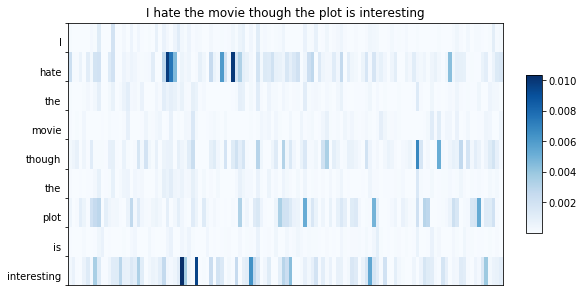
\includegraphics[width=\textwidth,height=\textheight,keepaspectratio]{figs/variance_plot.png}
  \caption{Plot of deviation from the mean of word vector components}
  \label{fig:var-fig}
\end{figure*}

I also employ a technique for visualising word vectors as heatmaps (Li et al. 2015) \cite{viz}. Each column shows the difference from the mean of each component in each word embedding. The influence of a word embedding is determined by its deviation from the mean vector, since these vectors will contribute more to learned document embeddings. From this, we can hypothesise that more importance is placed on key sentiment indicators - e.g. 'hate' or 'love'. In addition, words connecting clauses and negation words are salient, since they can change the meanings of parts of the document. An example of this is \ref{fig:var-fig}, in the phrase \textit{"I hate the movie, although the plot is interesting"}, where we can see that the words hate, although, plot and interesting are the most salient. Here, a negative clause is combined with a positive clause, with the overall class being negative since the use of 'hate' overshadows the 'interesting' plot. This can also be seen on the heatmap, with 'hate' being the more salient adjective.

\begin{figure*}
  \centering
  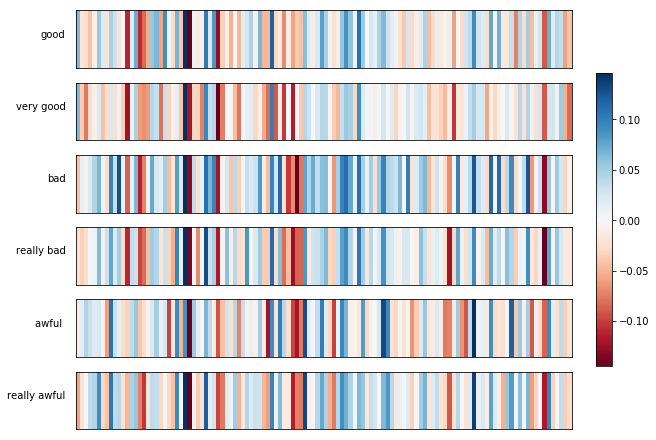
\includegraphics[width=\textwidth,height=\textheight,keepaspectratio]{figs/intense.png}
  \caption{Plot of document embeddings for phrases and their intensifications}
  \label{fig:intense-fig}
\end{figure*}

\begin{figure*}
  \centering
  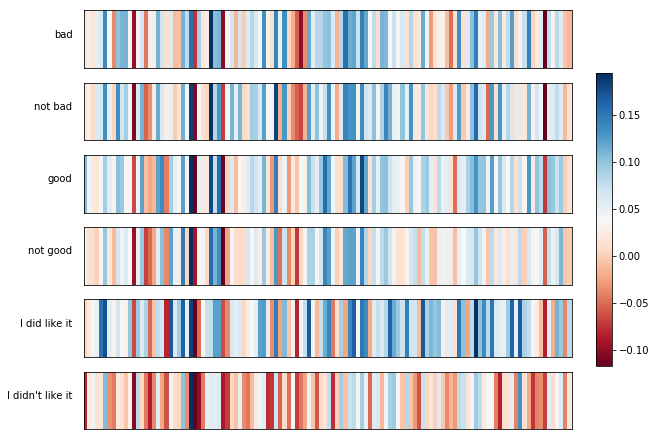
\includegraphics[width=\textwidth,height=\textheight,keepaspectratio]{figs/negate.png}
  \caption{Plot of document embeddings for phrases and their negations}
  \label{fig:negate-fig}
\end{figure*}


We can also visualise entire document vectors as heatmaps. This allows us to see the effect of intensification and negation on document vectors. Figures \ref{fig:intense-fig} and \ref{fig:negate-fig} show the document vectors for several short phrases and their modifications. Some patterns can be seen (qualitatively) here, with certain dimensions changing on modification, for example the one highlighted on the figure. Here, intensification should lead to a classification with higher confidence, and negation to the opposite classification.

% The T-SNE projection in figure \ref{} also shows how doc2vec learns how negation affects documents. Negations of positive phrases  are seen to be close to negative phrases - e.g. 'not good' is closer to 'bad' than to 'good'.

\section{Conclusion}


I have shown that doc2vec produces a representation, that when paired with an SVM model, can outperform a bag-of-words representation. Despite not being directly interpretable, doc2vec still creates a meaningful semantic space for documents (analogously to word2vec), and we can visualise vectors in this space to show this.

\end{multicols}
\clearpage
\bibliography{refs}




\end{document}
